% Options for packages loaded elsewhere
\PassOptionsToPackage{unicode}{hyperref}
\PassOptionsToPackage{hyphens}{url}
%
\documentclass[
  11pt,
  ignorenonframetext,
]{beamer}
\usepackage{pgfpages}
\setbeamertemplate{caption}[numbered]
\setbeamertemplate{caption label separator}{: }
\setbeamercolor{caption name}{fg=normal text.fg}
\beamertemplatenavigationsymbolsempty
% Prevent slide breaks in the middle of a paragraph
\widowpenalties 1 10000
\raggedbottom
\setbeamertemplate{part page}{
  \centering
  \begin{beamercolorbox}[sep=16pt,center]{part title}
    \usebeamerfont{part title}\insertpart\par
  \end{beamercolorbox}
}
\setbeamertemplate{section page}{
  \centering
  \begin{beamercolorbox}[sep=12pt,center]{part title}
    \usebeamerfont{section title}\insertsection\par
  \end{beamercolorbox}
}
\setbeamertemplate{subsection page}{
  \centering
  \begin{beamercolorbox}[sep=8pt,center]{part title}
    \usebeamerfont{subsection title}\insertsubsection\par
  \end{beamercolorbox}
}
\AtBeginPart{
  \frame{\partpage}
}
\AtBeginSection{
  \ifbibliography
  \else
    \frame{\sectionpage}
  \fi
}
\AtBeginSubsection{
  \frame{\subsectionpage}
}
\usepackage{amsmath,amssymb}
\usepackage{lmodern}
\usepackage{iftex}
\ifPDFTeX
  \usepackage[T1]{fontenc}
  \usepackage[utf8]{inputenc}
  \usepackage{textcomp} % provide euro and other symbols
\else % if luatex or xetex
  \usepackage{unicode-math}
  \defaultfontfeatures{Scale=MatchLowercase}
  \defaultfontfeatures[\rmfamily]{Ligatures=TeX,Scale=1}
\fi
% Use upquote if available, for straight quotes in verbatim environments
\IfFileExists{upquote.sty}{\usepackage{upquote}}{}
\IfFileExists{microtype.sty}{% use microtype if available
  \usepackage[]{microtype}
  \UseMicrotypeSet[protrusion]{basicmath} % disable protrusion for tt fonts
}{}
\makeatletter
\@ifundefined{KOMAClassName}{% if non-KOMA class
  \IfFileExists{parskip.sty}{%
    \usepackage{parskip}
  }{% else
    \setlength{\parindent}{0pt}
    \setlength{\parskip}{6pt plus 2pt minus 1pt}}
}{% if KOMA class
  \KOMAoptions{parskip=half}}
\makeatother
\usepackage{xcolor}
\newif\ifbibliography
\usepackage{graphicx}
\makeatletter
\def\maxwidth{\ifdim\Gin@nat@width>\linewidth\linewidth\else\Gin@nat@width\fi}
\def\maxheight{\ifdim\Gin@nat@height>\textheight\textheight\else\Gin@nat@height\fi}
\makeatother
% Scale images if necessary, so that they will not overflow the page
% margins by default, and it is still possible to overwrite the defaults
% using explicit options in \includegraphics[width, height, ...]{}
\setkeys{Gin}{width=\maxwidth,height=\maxheight,keepaspectratio}
% Set default figure placement to htbp
\makeatletter
\def\fps@figure{htbp}
\makeatother
\setlength{\emergencystretch}{3em} % prevent overfull lines
\providecommand{\tightlist}{%
  \setlength{\itemsep}{0pt}\setlength{\parskip}{0pt}}
\setcounter{secnumdepth}{-\maxdimen} % remove section numbering
\newlength{\cslhangindent}
\setlength{\cslhangindent}{1.5em}
\newlength{\csllabelwidth}
\setlength{\csllabelwidth}{3em}
\newlength{\cslentryspacingunit} % times entry-spacing
\setlength{\cslentryspacingunit}{\parskip}
\newenvironment{CSLReferences}[2] % #1 hanging-ident, #2 entry spacing
 {% don't indent paragraphs
  \setlength{\parindent}{0pt}
  % turn on hanging indent if param 1 is 1
  \ifodd #1
  \let\oldpar\par
  \def\par{\hangindent=\cslhangindent\oldpar}
  \fi
  % set entry spacing
  \setlength{\parskip}{#2\cslentryspacingunit}
 }%
 {}
\usepackage{calc}
\newcommand{\CSLBlock}[1]{#1\hfill\break}
\newcommand{\CSLLeftMargin}[1]{\parbox[t]{\csllabelwidth}{#1}}
\newcommand{\CSLRightInline}[1]{\parbox[t]{\linewidth - \csllabelwidth}{#1}\break}
\newcommand{\CSLIndent}[1]{\hspace{\cslhangindent}#1}
%---------------------------------------------------------------------------
% BeamerHead.sty
%---------------------------------------------------------------------------
\usepackage{ifxetex,ifluatex}

%---------------------------------------------------------------------------
% General
%---------------------------------------------------------------------------
\usepackage{setspace}
\setstretch{1.25}

%\usepackage[T1]{fontenc} % Use 8-bit encoding that has 256 glyphs
% \usepackage[utf8]{inputenc}
% \usepackage{lmodern}

%\usepackage{fourier} % Use the Adobe Utopia font for the document - comment this line to return to the LaTeX default

% \setbeamerfont{item}{size*={7.5}{8}}
% \setbeamerfont{item projected}{size*={7.5}{8}}
% \setbeamerfont{itemize item}{size*={7.5}{8}}
% \setbeamerfont{itemize subitem}{size*={7.5}{8}}
% \setbeamerfont{itemize subsubitem}{size*={7.5}{8}}
% \setbeamerfont{itemize/enumerate body}{size*={7.5}{8}}
% \setbeamerfont{itemize/enumerate subbody}{size*={7.5}{8}}
% \setbeamerfont{itemize/enumerate subsubbody}{size*={7.5}{8}}
% \setbeamerfont{caption}{size*={7.5}{8}}
% \setbeamerfont{caption name}{size*={7.5}{8}}
% \setbeamerfont{frametitle}{size*={9}{9.5}}
% \setbeamerfont{normal text}{size*={7.5}{8}}
% Smaller itemize bullets
\setbeamertemplate{itemize items}{
	\raisebox{0.15\height}{$\vcenter{\hbox{\scalebox{0.5}{
	\usebeamercolor[fg]{structure} $\blacktriangleright$}}}$}}

% sans serif math accents
\usepackage{sansmathaccent}

% % Small font in shaded environment
% \renewenvironment{Shaded}{\begin{snugshade}\small}{\end{snugshade}}

%\usepackage{sectsty} % Allows customizing section commands
%\allsectionsfont{\centering \normalfont\scshape} % Make all sections centered, the default font and small caps
%\numberwithin{equation}{section} % Number equations within sections
%\numberwithin{figure}{section} % Number figures within sections
%\numberwithin{table}{section} % Number tables within sections

\usepackage{multicol}
\setlength{\columnsep}{20pt}
\newlength\Colsep

%---------------------------------------------------------------------------
% Header/footer
%---------------------------------------------------------------------------
\setbeamertemplate{navigation symbols}{}
\setbeamertemplate{footline}[page number]

%---------------------------------------------------------------------------
% Citations
%---------------------------------------------------------------------------
% \usepackage[backend=bibtex]{biblatex}

%---------------------------------------------------------------------------
% Tables, figures, images
%---------------------------------------------------------------------------
\usepackage{wrapfig}
\usepackage{longtable}
\setlength{\LTcapwidth}{\textwidth}
\usepackage{xtab, booktabs}
\usepackage{multirow}

% \usepackage{tikz}% Probability trees and flow charts and the like
% \usetikzlibrary{%
% trees,
% arrows,
% shapes,
% %decoration,
% automata,
% backgrounds,
% petri}

% Witin cell wrapping
% https://tex.stackexchange.com/questions/2441/how-to-add-a-forced-line-break-inside-a-table-cell
\usepackage{makecell}
\renewcommand\theadalign{bc}
\renewcommand\theadfont{\bfseries}
\renewcommand\theadgape{\Gape[4pt]}
\renewcommand\cellgape{\Gape[4pt]}
% Usage
% \thead{Two line \\ head}
% \makecell{Some really \\ longer text}

% \usepackage{graphicx,grffile}
% For tables and figures in parts %%%%
\usepackage{caption}
\DeclareCaptionLabelFormat{cont}{#1~#2\alph{ContinuedFloat}}
% \usepackage{subcaption}
% \captionsetup{font=scriptsize,labelfont=scriptsize}
%\graphicspath{ {file.path.here} }

% \usepackage{subfloat}

% Set column widths in tabular environment!
\usepackage{array}
\newcommand{\PreserveBackslash}[1]{\let\temp=\\#1\let\\=\temp}
\newcolumntype{C}[1]{>{\PreserveBackslash\centering}p{#1}}
\newcolumntype{R}[1]{>{\PreserveBackslash\raggedleft}p{#1}}
\newcolumntype{L}[1]{>{\PreserveBackslash\raggedright}p{#1}}

% Fancy fit image command with optional caption
\usepackage{adjustbox} % Shrink stuff
% \usepackage{showframe} % Useful for debugging

%---------------------------------------------------------------------------
% Typographical addendum
%---------------------------------------------------------------------------
\usepackage{bbm} % more BB
\input{\string~/HeadRs/common_supplement.tex}

% https://tex.stackexchange.com/questions/136143/tikz-animated-figure-in-beamer
\tikzset{
  invisible/.style={opacity=0},
  visible on/.style={alt={#1{}{invisible}}},
  alt/.code args={<#1>#2#3}{%
    \alt<#1>{\pgfkeysalso{#2}}{\pgfkeysalso{#3}} % \pgfkeysalso doesn't change the path
  },
}
\setlength{\itemindent}{0em}
\setlength{\leftmargini}{1em}
\setlength{\leftmarginii}{1em}
\setlength{\leftmarginiii}{1em}
\usepackage{bbold}
\ifLuaTeX
  \usepackage{selnolig}  % disable illegal ligatures
\fi
\IfFileExists{bookmark.sty}{\usepackage{bookmark}}{\usepackage{hyperref}}
\IfFileExists{xurl.sty}{\usepackage{xurl}}{} % add URL line breaks if available
\urlstyle{same} % disable monospaced font for URLs
\hypersetup{
  pdftitle={Evaluating hypothetical limits on metalworking fluid exposure for reducing non-Hodgkin lymphoma incidence},
  hidelinks,
  pdfcreator={LaTeX via pandoc}}

\title{Evaluating hypothetical limits on metalworking fluid exposure for
reducing non-Hodgkin lymphoma incidence}
\subtitle{An application of the hazard-extended parametric g-formula}
\author{}
\date{\vspace{-2.5em}\today}

\begin{document}
\frame{\titlepage}

\begin{frame}{Non-Hodgkin Lymphoma}
\protect\hypertarget{non-hodgkin-lymphoma}{}
\begin{itemize}
\tightlist
\item
  7th most common cancer in the US
\item
  Incidence rose dramatically 1960 to 1990 around the world

  \begin{itemize}
  \tightlist
  \item
    In the US: 8.5 to 18.3 per 100,000 between 1973 and 2019
  \end{itemize}
\item
  Strongest risk factors\textsuperscript{1}

  \begin{itemize}
  \tightlist
  \item
    Immunosuppression, both genetic and acquired
  \item
    Infection by \emph{H. pylori}, Epstein-Barr virus, Hepatitis C
    virus, HIV
  \end{itemize}
\item
  Known risk factors account for about 50\% of observed
  incidence\textsuperscript{2}
\end{itemize}

\note{
In order of frequency (2020):
1. breast
2. lung/bronchus
3. prostate
4. colorectal
5. melanoma
6. bladder
7. NHL
8. kidney \& renal pelvis,
9. endometrial
10. leukemia
}
\end{frame}

\begin{frame}{NHL and peseticides}
\protect\hypertarget{nhl-and-peseticides}{}
\begin{itemize}
\tightlist
\item
  Rise in NHL mirrors rise in chemicalization of agriculture, industry,
  and warfare\textsuperscript{3}

  \begin{itemize}
  \tightlist
  \item
    Agricultural exposure to pesticides very well studied
  \item
    Meta-analyses yielded consistent associations with pesticides:\\
    carbamate, organophosphorous, triazine,
    organochlorine\textsuperscript{4}
  \end{itemize}
\end{itemize}

\begin{center}
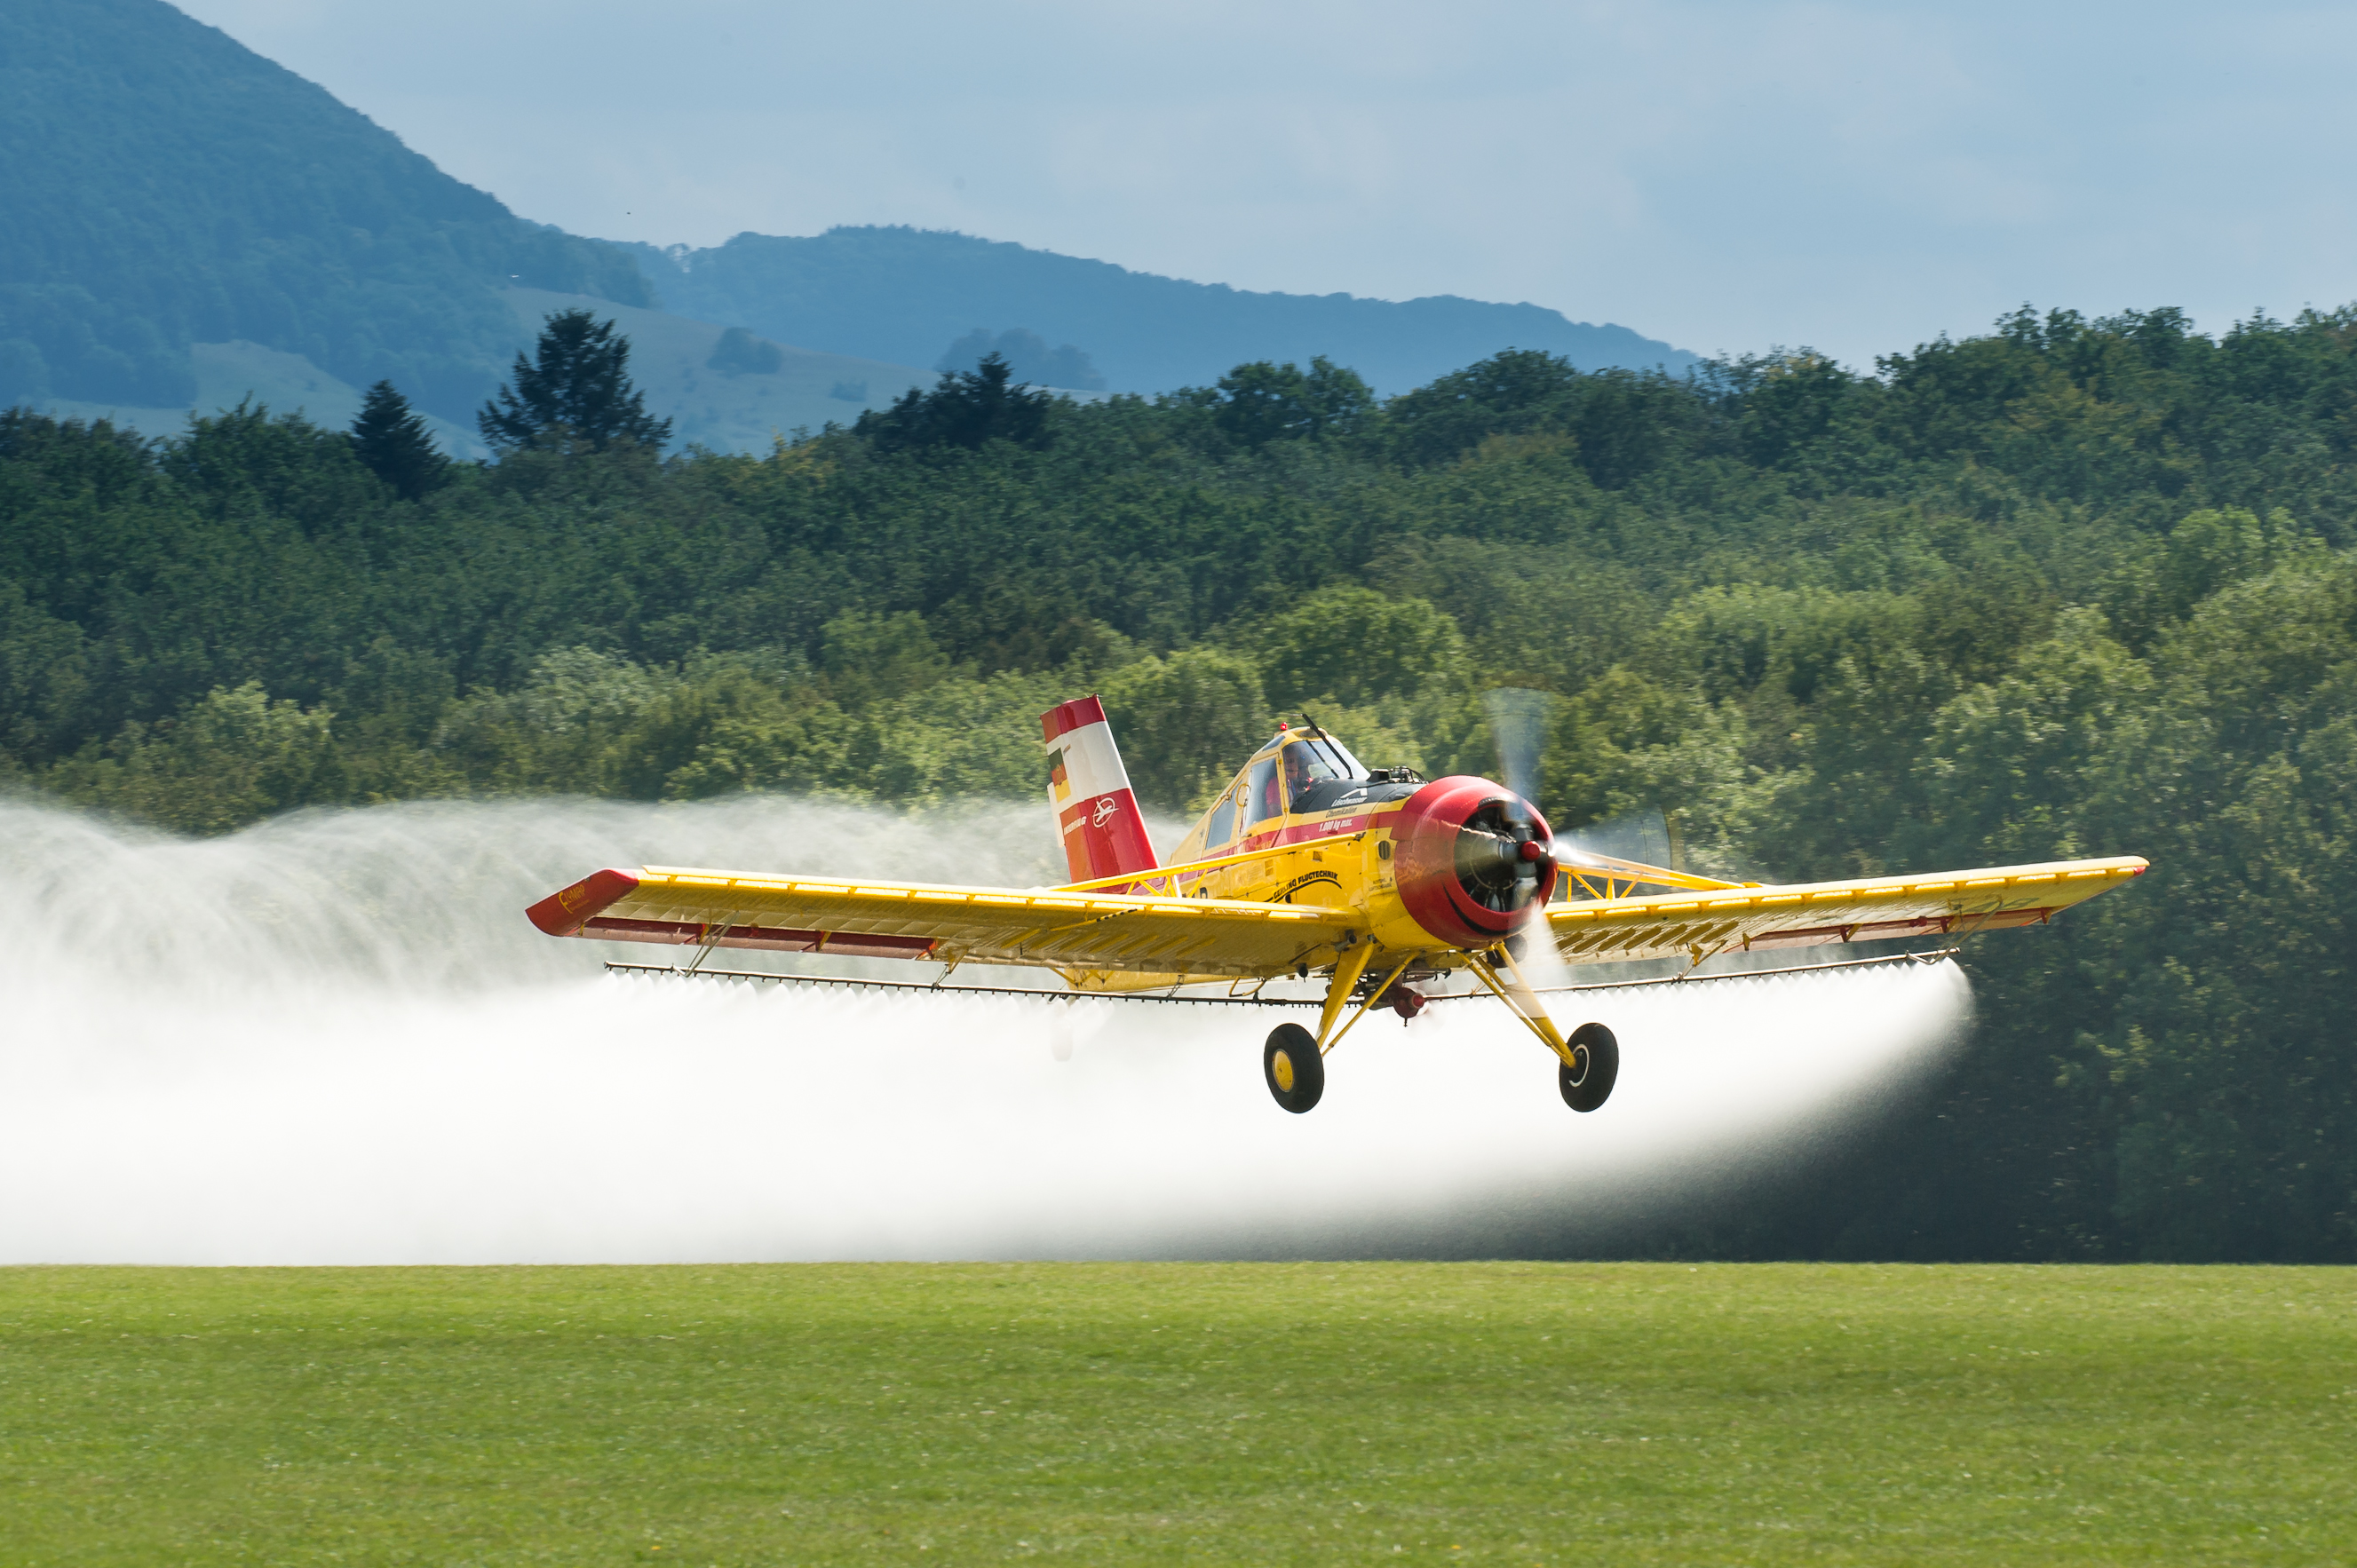
\includegraphics[width=2in]{./resources/pesticide_aircraft.jpg}
\end{center}

\note{
Several organophosphorous pesticides considered possibly carcinogenic by IARC
Several chlorinated solvents are IARC Group 1 carcinogens
}
\end{frame}

\begin{frame}{Soluble MWF}
\protect\hypertarget{soluble-mwf}{}
\begin{itemize}
\tightlist
\item
  Water-based soluble MWFs contain diverse additives:\\

  \begin{itemize}
  \tightlist
  \item
    Triazines: biocides
  \item
    Nitrites: rust inhibitors
  \item
    Sulfonates: emulsifiers
  \item
    Organochlorines: extreme pressure performance enhancers
  \end{itemize}
\item
  In UAW-GM, soluble MWF was used more frequently and in much larger
  quantities than straight and synthetic MWF
\item
  Globally, soluble MWF is the most common
\end{itemize}
\end{frame}

\begin{frame}{MWF exposure in UAW-GM}
\protect\hypertarget{mwf-exposure-in-uaw-gm}{}
\begin{figure}
\centering
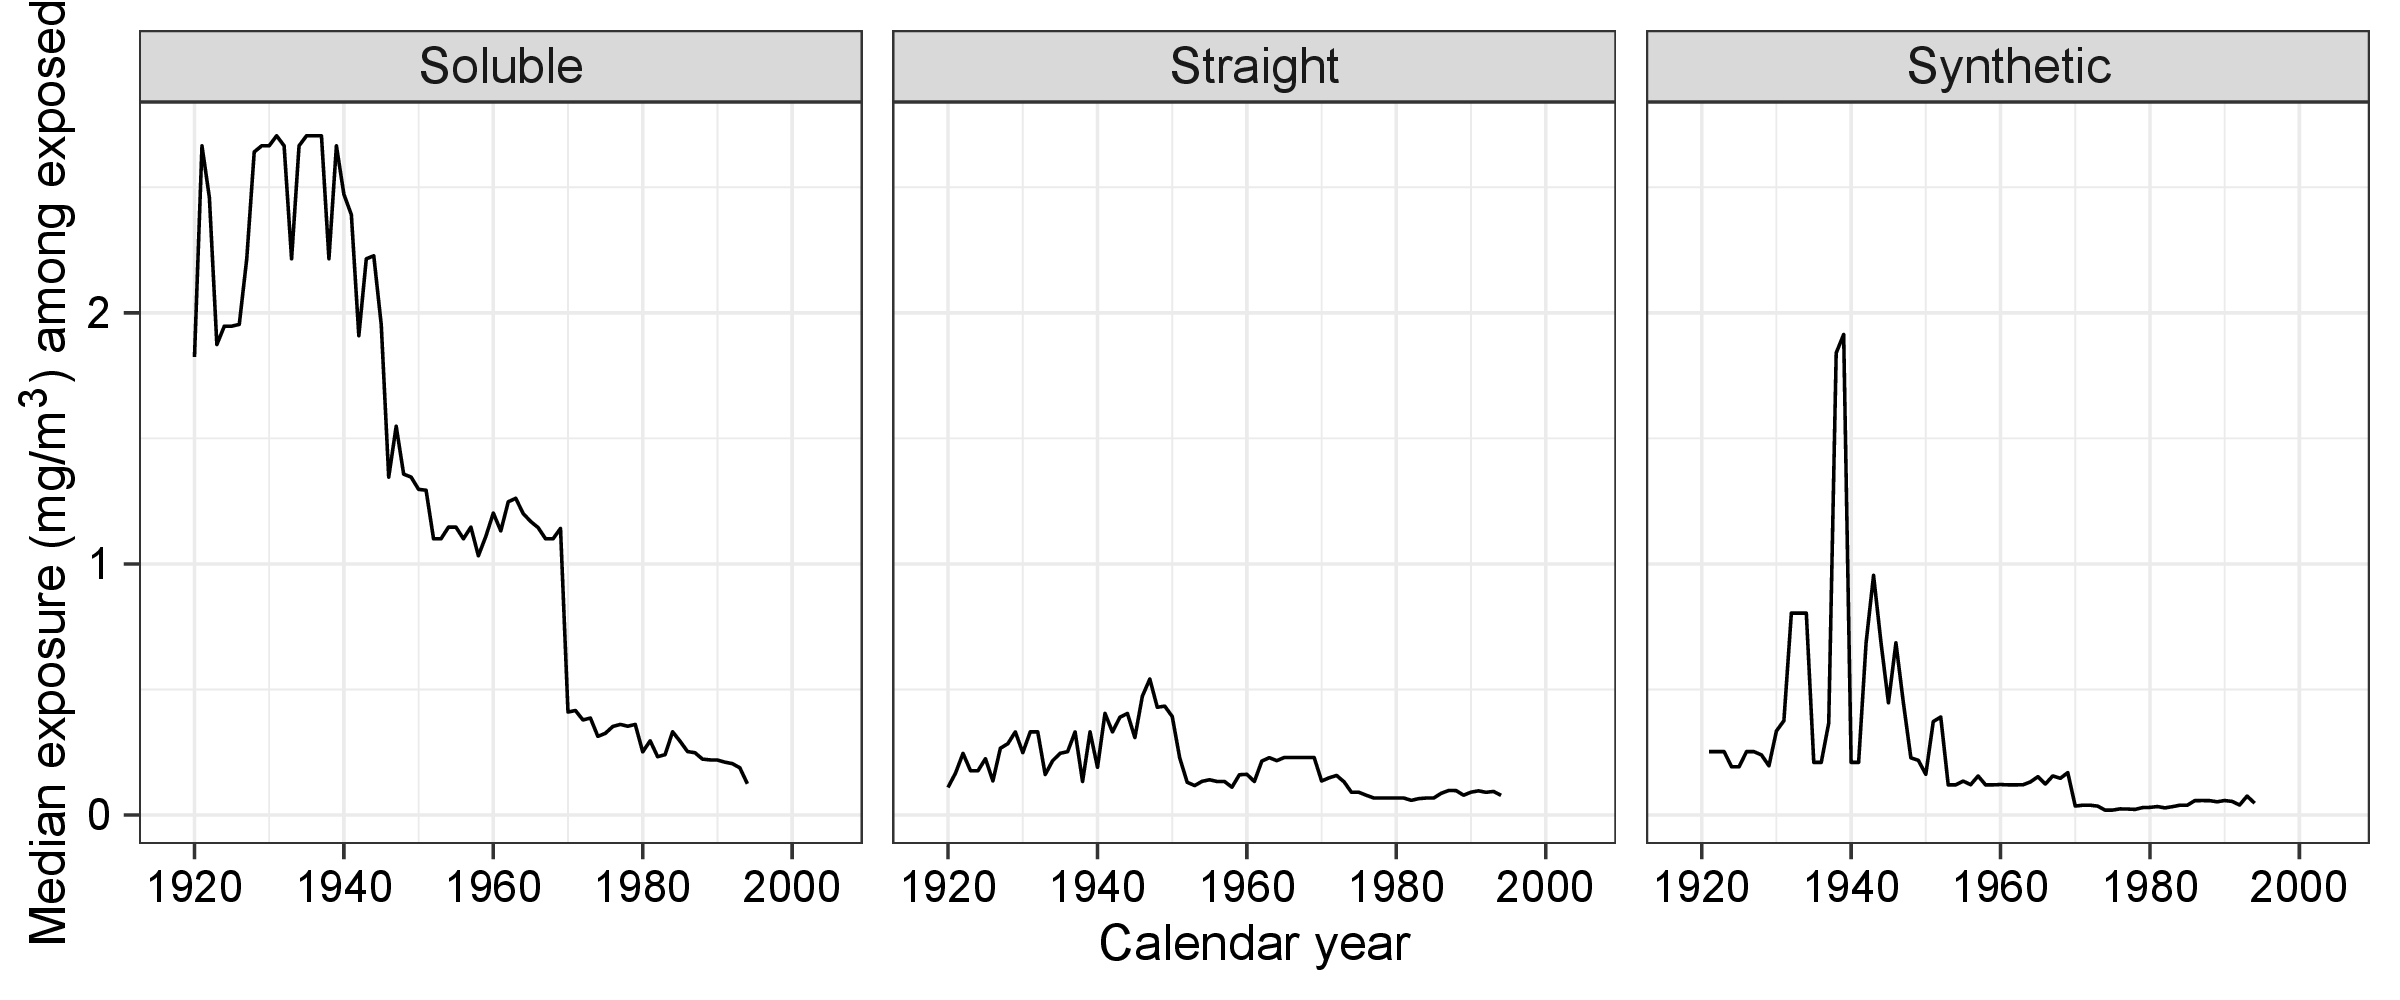
\includegraphics[width=4in,height=\textheight]{/Users/kevinchen/eisen/gm-nhl-ice/resources/images/exposure.png}
\caption{Median average annual exposure among exposed workers over
time.}
\end{figure}

\begin{itemize}
\tightlist
\item
  89\% ever exposed to soluble
\item
  57\% ever exposed to straight
\item
  35\% ever exposed to synthetic
\end{itemize}
\end{frame}

\begin{frame}{MWF exposure and NHL in UAW-GM}
\protect\hypertarget{mwf-exposure-and-nhl-in-uaw-gm}{}
\begin{figure}
\centering
\includegraphics[width=4in,height=\textheight]{/Users/kevinchen/eisen/gm-nhl-ice/../gm-cancer-inc/reports/resources/Lag 21/subplots/AJE-01232-2021 Colbeth Figure 2N.pdf}
\caption{NHL and soluble MWF exposure in recent cancer incidence
analysis (Hilary's paper, in press).}
\end{figure}
\end{frame}

\begin{frame}{Iterated conditional expectation (ICE) g-formula}
\protect\hypertarget{iterated-conditional-expectation-ice-g-formula}{}
ICE g-formula estimators rely on the tower property of expectation (from
law of total probability)

\begin{itemize}
\tightlist
\item
  For example,
  \(\mathbb E\, \mathbb E \left[Y \mid A = \check{a}, W \right] = \mathbb E \left[Y \mid A = \check{a}\right]\)
\item
  For discrete \(W\), we have\\
  \(\mathbb E \left[Y \mid A = \check{a}\right] = \sum_{w \in \mathcal W} \mathbb E\, \left[Y \mid A = \check{a}, W = w\right] \Prob{W = w}\)\\
  This is the non-parametric \(g\)-computation result, which we can
  estimate parametrically by specifying a model:

  \begin{center}$\mathbb E\left[Y \mid A = \check{a}, W = w\right] = \beta_0 + \beta_1 \check{a} + \beta_2 w$\end{center}

  \begin{itemize}
  \tightlist
  \item
    Avoids the need for propensity score
  \item
    Relies heavily on correct model specification
  \item
    Equivalent to model-based standardization
  \end{itemize}
\end{itemize}
\end{frame}

\begin{frame}{ICE g-formula for multiple timepoints}
\protect\hypertarget{ice-g-formula-for-multiple-timepoints}{}
\footnotesize\renewcommand{\arraystretch}{1.2}
\begin{tabular}{ll}
Put & $\psi =  \E[f_{Y_J}]{Y_J(1 - Y_{J - 1}) \mid \bar L_{J}, \bar A_{J} = \bar A^g_{J}, \bar Y_{J - 1} = C_J = 0}$ \\
Put & $\psi =  \E[f_{L_{J}}]{\,\psi\, \mid \bar L_{J - 1}, \bar A_{J - 1} = \bar A^g_{J - 1}, \bar Y_{J - 1} = C_{J} = 0}$ \\
Put & $\psi =  \E[f_{Y_{J - 1}}]{Y_{J - 1} (1 - Y_{J - 2}) + \,\psi\, \mid \bar L_{J - 1}, \bar A_{J - 1} = \bar A^g_{J - 1}, \bar Y_{J - 2} = C_{J - 1} = 0}$ \\
& $\hspace{4pt} \vdots$ \\
Put & $\psi =  \E[f_{Y_1}]{Y_1 + \,\psi\, \mid L_1, A_1 = A^g_1, \bar Y_{0} = C_0 = 0}$ \\
\\
$\leadsto$ &  $\E{Y^g_J} =  \E[f_{L_{1}}]{\,\psi\,}$
\end{tabular}

For \emph{hazard-extended} ICE g-formula,\\
we use discrete hazard estimate for interval \((j - 1, j]\) in place of
\(Y_j\)
\end{frame}

\begin{frame}{Intervention of interest}
\protect\hypertarget{intervention-of-interest}{}
\begin{itemize}
\tightlist
\item
  Deterministic stochastic interventions: limit soluble MWF to\\

  \begin{itemize}
  \tightlist
  \item
    0.5 mg/m\textsuperscript{3} (NIOSH REL)
  \item
    0.25 mg/m\textsuperscript{3}
  \item
    0.05 mg/m\textsuperscript{3}
  \end{itemize}
\item
  Dynamic stochastic interventions: reduce soluble MWF such that total
  MWF exposure limited to 0.5, 0.25, and 0.05 mg/m\textsuperscript{3}

  \begin{itemize}
  \tightlist
  \item
    Translates to the following exposure limits on soluble MWF:

    \begin{itemize}
    \tightlist
    \item
      \(\max\left(0,\ 0.5 - \text{str} - \text{syn}\right)\)
    \item
      \(\max\left(0,\ 0.25 - \text{str} - \text{syn}\right)\)
    \item
      \(\max\left(0,\ 0.05 - \text{str} - \text{syn}\right)\)
    \end{itemize}
  \end{itemize}
\end{itemize}
\end{frame}

\begin{frame}{Illustration of interventions when applied}
\protect\hypertarget{illustration-of-interventions-when-applied}{}
\begin{figure}
\centering
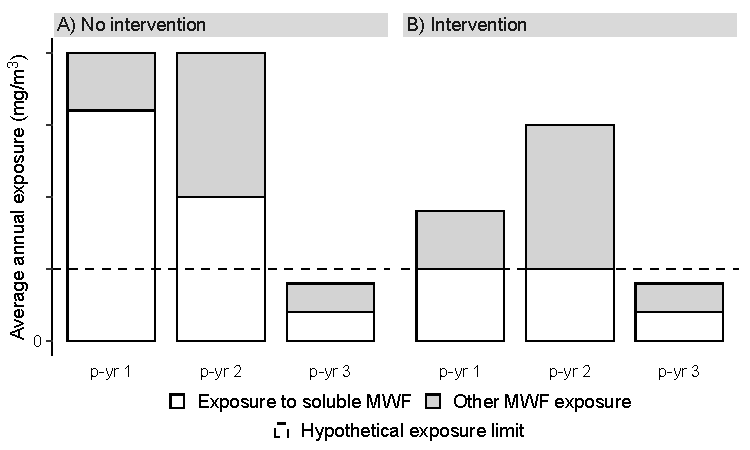
\includegraphics[width=4.25in,height=\textheight]{/Users/kevinchen/eisen/gm-nhl-ice/resources/interventions.pdf}
\caption{Observed and post-intervention levels of exposure in three
example person-years.}
\end{figure}
\end{frame}

\begin{frame}{Results}
\protect\hypertarget{results}{}
\scriptsize\setlength{\tabcolsep}{3pt}
\begin{table}[ht]
\centering
\begin{tabular}{p{0.27\linewidth}C{0.18\linewidth}C{0.1\linewidth}ccc}
  \hline
Exposure limit on soluble MWF (mg/m$^3$) & Person-years intervened (\%) & Risk per 1000 & (risk 95\% CI) & RR & (RR 95\% CI) \\ 
  \hline
None & 0.0 & 9.56 & (8.15, 10.89) & 1.00 &  \\ 
  0.5 & 23.8 & 8.30 & (6.52, 10.19) & 0.87 & (0.72, 1.02) \\ 
  0.25 & 36.2 & 8.06 & (6.15, 10.15) & 0.84 & (0.68, 1.01) \\ 
  0.05 & 43.9 & 7.52 & (5.73, 9.51) & 0.79 & (0.62, 0.97) \\ 
  max(0, 0.5 – str – syn) & 28.3 & 8.00 & (6.27, 9.87) & 0.84 & (0.69, 0.99) \\ 
  max(0, 0.25 – str – syn) & 40.0 & 7.69 & (5.88, 9.64) & 0.80 & (0.64, 0.98) \\ 
  max(0, 0.05 – str – syn) & 52.8 & 6.89 & (4.62, 9.75) & 0.72 & (0.48, 1.01) \\ 
   \hline
\end{tabular}
\end{table}
\end{frame}

\begin{frame}{Discussion}
\protect\hypertarget{discussion}{}
\begin{itemize}
\tightlist
\item
  Assumption of correct model specification is doing heavy duty

  \begin{itemize}
  \tightlist
  \item
    Trade-off between satisfying positivity and correct model
    specification
  \item
    But approach is much more flexible than Cox PH
  \end{itemize}
\item
  Why bother with stochastic intervention?

  \begin{itemize}
  \tightlist
  \item
    In reality, companies may not reduce exposures already below REL
  \item
    In estimation, we can achieve positivity more easily
  \end{itemize}
\item
  Why bother with complex \emph{dynamic} stochastic intervention

  \begin{itemize}
  \tightlist
  \item
    NIOSH REL is for total MWF exposure?
  \item
    Dynamic interventions can achieve risk reductions by intervening on
    fewer person-years (analytically) and processes (in reality)
  \end{itemize}
\end{itemize}
\end{frame}

\begin{frame}{Citations}
\protect\hypertarget{citations}{}
\singlespacing\footnotesize

\hypertarget{refs}{}
\begin{CSLReferences}{0}{0}
\leavevmode\vadjust pre{\hypertarget{ref-Ekstrom-Smedby_2006}{}}%
\CSLLeftMargin{1. }%
\CSLRightInline{Ekström-Smedby K. Epidemiology and etiology of
non-{Hodgkin} lymphoma--a review. \emph{Acta oncologica}.
2006;45(3):258-271.}

\leavevmode\vadjust pre{\hypertarget{ref-Hartge_1992}{}}%
\CSLLeftMargin{2. }%
\CSLRightInline{Hartge P, Devesa SS. Quantification of the impact of
known risk factors on time trends in non-hodgkin's lymphoma incidence.
\emph{Cancer research}. 1992;52(19\_Supplement):5566s-5569s.}

\leavevmode\vadjust pre{\hypertarget{ref-Nelson_2005}{}}%
\CSLLeftMargin{3. }%
\CSLRightInline{Nelson NJ. Studies examine whether persistent organic
agents may be responsible for rise in lymphoma rates. \emph{Journal of
the National Cancer Institute}. 2005;97(20):1490-1491.}

\leavevmode\vadjust pre{\hypertarget{ref-Schinasi_2014}{}}%
\CSLLeftMargin{4. }%
\CSLRightInline{Schinasi L, Leon ME. Non-{Hodgkin} lymphoma and
occupational exposure to agricultural pesticide chemical groups and
active ingredients: A systematic review and meta-analysis.
\emph{International Journal of Environmental Research and Public
Health}. 2014;11(4):4449-4527.
doi:\href{https://doi.org/10.3390/ijerph110404449}{10.3390/ijerph110404449}.}

\end{CSLReferences}
\end{frame}

\end{document}
